  \documentclass[11pt]{article}
\usepackage[french]{babel}

\usepackage[utf8]{inputenc}
\usepackage{palatino}
\usepackage[T1]{fontenc}


\usepackage{url}
\usepackage{amsmath}

\usepackage[top=2cm,bottom=2cm,left=2.1cm,right=2.1cm,headsep=10pt,a4paper]{geometry}
\usepackage{fancyhdr}


\usepackage{graphicx,float} % figure et placement de figure
\usepackage{listings} %%inclusion de programmes
\usepackage{enumitem} 
\usepackage[french]{babel}
\frenchbsetup{StandardLists=true} 

\lstset{
  language=C++,
  basicstyle=\ttfamily\small, %
  identifierstyle=\color{black}, %
  keywordstyle=\color{blue}, %
  stringstyle=\color{blue}, %
  commentstyle=\it\color{green}, %
}

\usepackage{xcolor}

\pagestyle{fancy}
\lhead{}
\chead{\fontsize{10}{10}{Mif24 - UCBL - 2013/2014}}
\rhead{\thepage}
\lfoot{\fontsize{10}{10}{Rapport Chemier, Duhamel, Farges}}

\renewcommand{\headrulewidth}{0pt}
\renewcommand{\footrulewidth}{0pt}


 \author{\fontsize{14}{14}{\bf Aurélien CHEMIER, Arnaud DUHAMEL, Maëlyss FARGES}}
 \title{\fontsize{16}{16}{{\bf Rapport MIF24}}}
 \date{\fontsize{11}{11}{2013/2014}}

\begin{document}

  \thispagestyle{empty}
  \maketitle
  \newpage
  \tableofcontents
  
  
  \newpage

  \section{Introduction}
    L'objectif de ce projet est d'implémenter un agent qui apprend à effectuer les interactions positives sans connaître à priori 
  son système motivationnel (\begin{math} mot_1 \end{math} ou \begin{math} mot_2 \end{math}) ni son environnement 
  (\begin{math}env_1\end{math} ou \begin{math}env_2\end{math}).
  
  
  \begin{itemize}
    \item Deux expériences sont possibles \begin{math} E = \{e_1,e_2\}\end{math}
    \item Deux résultats sont possibles \begin{math} R = \{r_1,r_2\} \end{math}
    \item Il y a donc quatre interactions possibles: \begin{math} E\times R=\{i_{11},i_{12},i_{21},i_{22}\}\end{math}
    
  \end{itemize}

    Pour coder l'agent nous avons utilisé le langage C++ et Qt.
    
  \section{Agent 1}
    \subsection{Description de l'agent}
    Les environnements sont :
      \begin{itemize}
      \item \begin{math} env_1: e_1 \Rightarrow r_1, e_2 \Rightarrow r_2 \end{math} 
      (\begin{math} i_{12}\end{math}  et \begin{math} i_{21}\end{math}  ne se produisent jamais).
      \item \begin{math} env_2:  e_1 \Rightarrow r_2, e_2 \Rightarrow r_1 \end{math} 
      (\begin{math} i_{11} \end{math} et \begin{math} i_{22}\end{math}  ne se produisent jamais).
      \end{itemize}
    Les Systèmes motivationnels sont:
      \begin{itemize}
      \item \begin{math} mot_1:  v(i_{11}) = v(i_{12}) = 1,v(i_{21}) = v(i_{22}) = -1\end{math}
      \item \begin{math} mot_2:  v(i_{11}) = v(i_{12}) = -1,v(i_{21}) = v(i_{22}) = 1 \end{math}
      \end{itemize}
      
      Concrètement, deux interactions donnent un résultat positif et deux autres donne un résultat positif.
    \subsection{Attributs}
      
      \begin{description}
	\item[m\_motivation] correspond au système de motivation de l'Agent tel qu'il a été décrit plus haut.	
	\item[m\_motivationScore] est la somme cumulée de tous les résultats d'expériences.
	\item[m\_trace] récupère toutes les effectuées par l'agent.
	\item[m\_environnement] est l'environnement dans lequel l'Agent évolue.
	\item[m\_exp] stocke les différentes expériences faite par l'Agent.
      \end{description}
    \subsection{Constructeur\textbackslash{}Destructeur}
    
    \lstinputlisting[caption={Constructeur et destructeur de l'Agent},language=C++,frame=single,firstline=3, lastline=23]{code/agent.cpp}
    
    \begin{description}
	\item[Le constructeur] initialise l'environnement avec l'environnement passé en paramètre et le score de motivation à 0.
	Il contrôle également le fichier trace.txt.
	\item[Le Destructeur] est vide.
      \end{description}
    
    
    \subsection{save()}
    
    \lstinputlisting[caption={Constructeur et destructeur de l'Agent},language=C++,frame=single,firstline=28, lastline=49]{code/agent.cpp}
    
    La fonction save() ajoute la dernière experience de l'agent dans le fichier trace.txt.
    
    \subsection{chooseResult()}
    
    \subsection{chooseExperience(const Resultat\& r)}
    
    \subsection{addMotivation(const Interaction\& i)}
    
  \section{Agent 2}
  \section{Agent 3}
  \section{Conclusion}

\end{document}


%\lstinputlisting[caption={Exemple de pointeur constant},language=C,frame=single]{Exemple/pointeurConstant.c}
%  \lstinputlisting[caption={Optimisation de l'exemple précédent},language=C,frame=single,firstline=6, lastline=6]{Exemple/mallocOpt.c}

 %\begin{figure}[H]
 %      \centering
  %     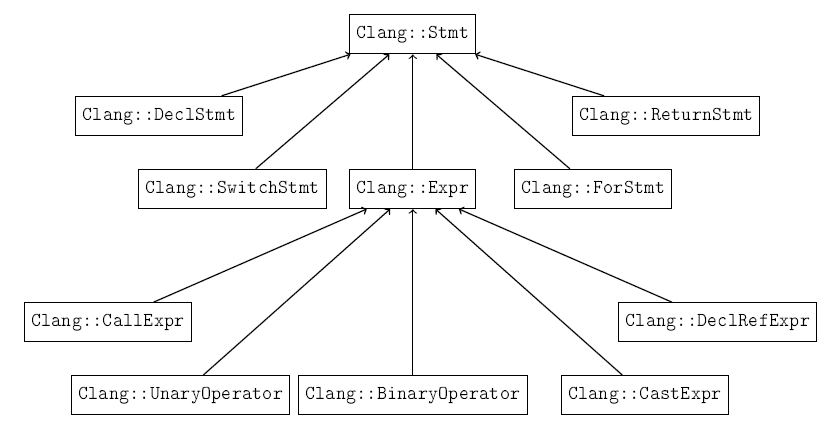
\includegraphics[scale=0.7]{soluce/graph.jpg} 
 %      \caption{Partie de l'architecture de Clang}
  %     \label{fig:graph}
  %   \end{figure}
